\section{Luthfi Muhammad Nabil(1174035)}
\subsection{Menginstalasi File Map Server}
Web Service yang digunakan pada map server ini adalah ms4w. Untuk melakukan instalasi mapserver, dibutuhkan file mapproxy yang dapat didownload dari \href{https://ms4w.com/}{Link MS4W}.
Berikut cara untuk instalasinya : 
\begin{enumerate}
    \item Pilih file zip Archive agar mudah untuk disetting dan semua file sudah tersedia
    \hfill\break
	\begin{figure}[H]
		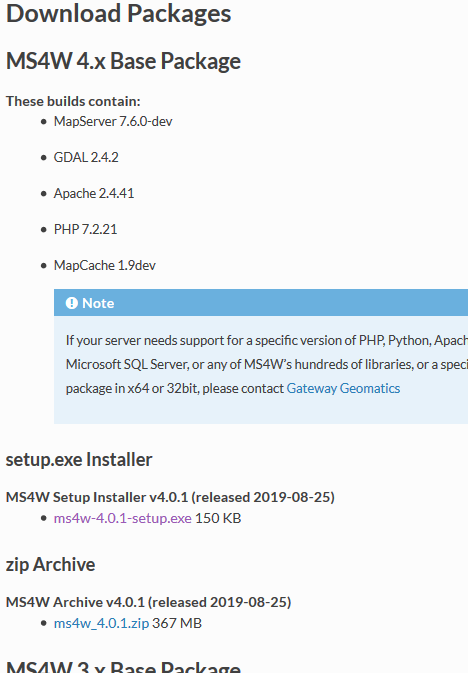
\includegraphics[width=8cm]{figures/1174035/tugas4/mapserver_1.png}
		\centering
		\caption{Download File}
	\end{figure}
    \item Extract file ms4w pada local disk System (Karena saya di C maka saya simpen di C)
    \hfill\break
	\begin{figure}[H]
		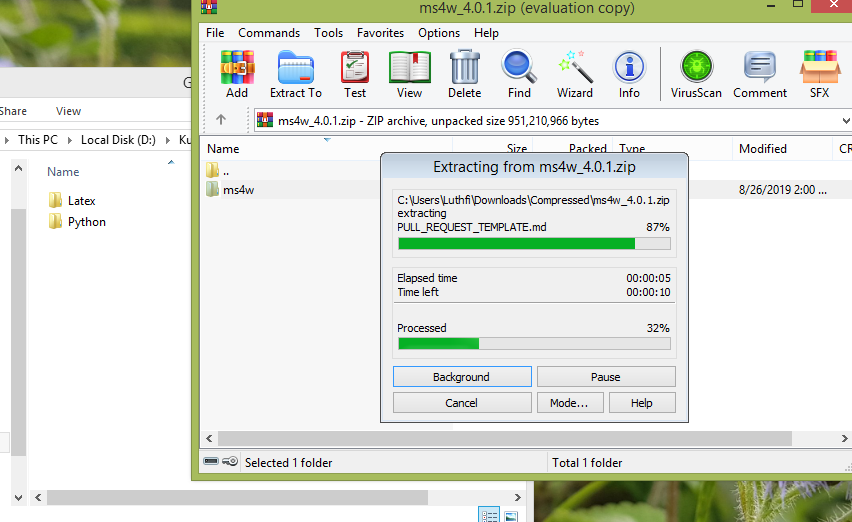
\includegraphics[width=8cm]{figures/1174035/tugas4/mapserver_2.png}
		\centering
		\caption{Extract File MS4W di Local Disk C}
	\end{figure}
    \item Masuk ke directory ms4w/apache/conf dan edit file httpd.conf. Jika anda perlu mengganti port saat map server dijalankan maka ganti port pada listen.
    \hfill\break
	\begin{figure}[H]
		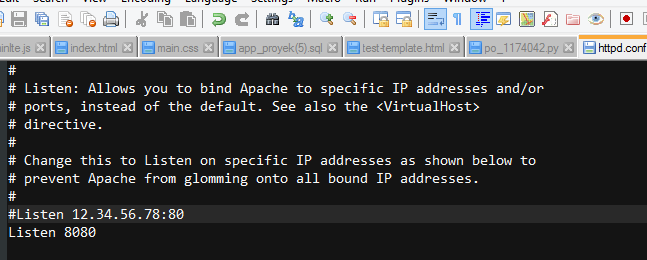
\includegraphics[width=8cm]{figures/1174035/tugas4/mapserver_3.png}
		\centering
		\caption{Ganti Port Apache Server pada MS4W}
	\end{figure}
    \item Pada directory yang sama, jalankan httpd.exe untuk dapat melihat hasil percobaan map server
    \hfill\break
	\begin{figure}[H]
		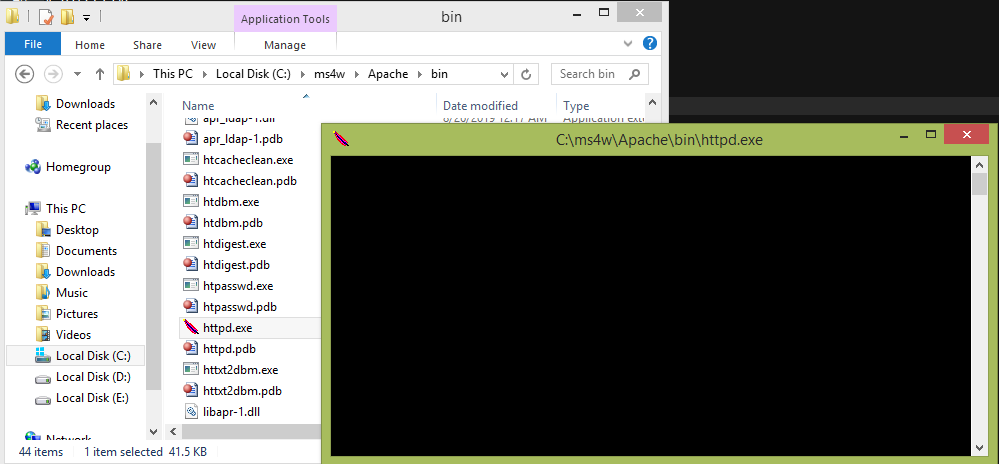
\includegraphics[width=8cm]{figures/1174035/tugas4/mapserver_4.png}
		\centering
		\caption{Menjalankan HTTPD.exe}
	\end{figure}
    \item Hasil yang dimunculkan adalah sebagai berikut untuk percobaan.
    \hfill\break
	\begin{figure}[H]
		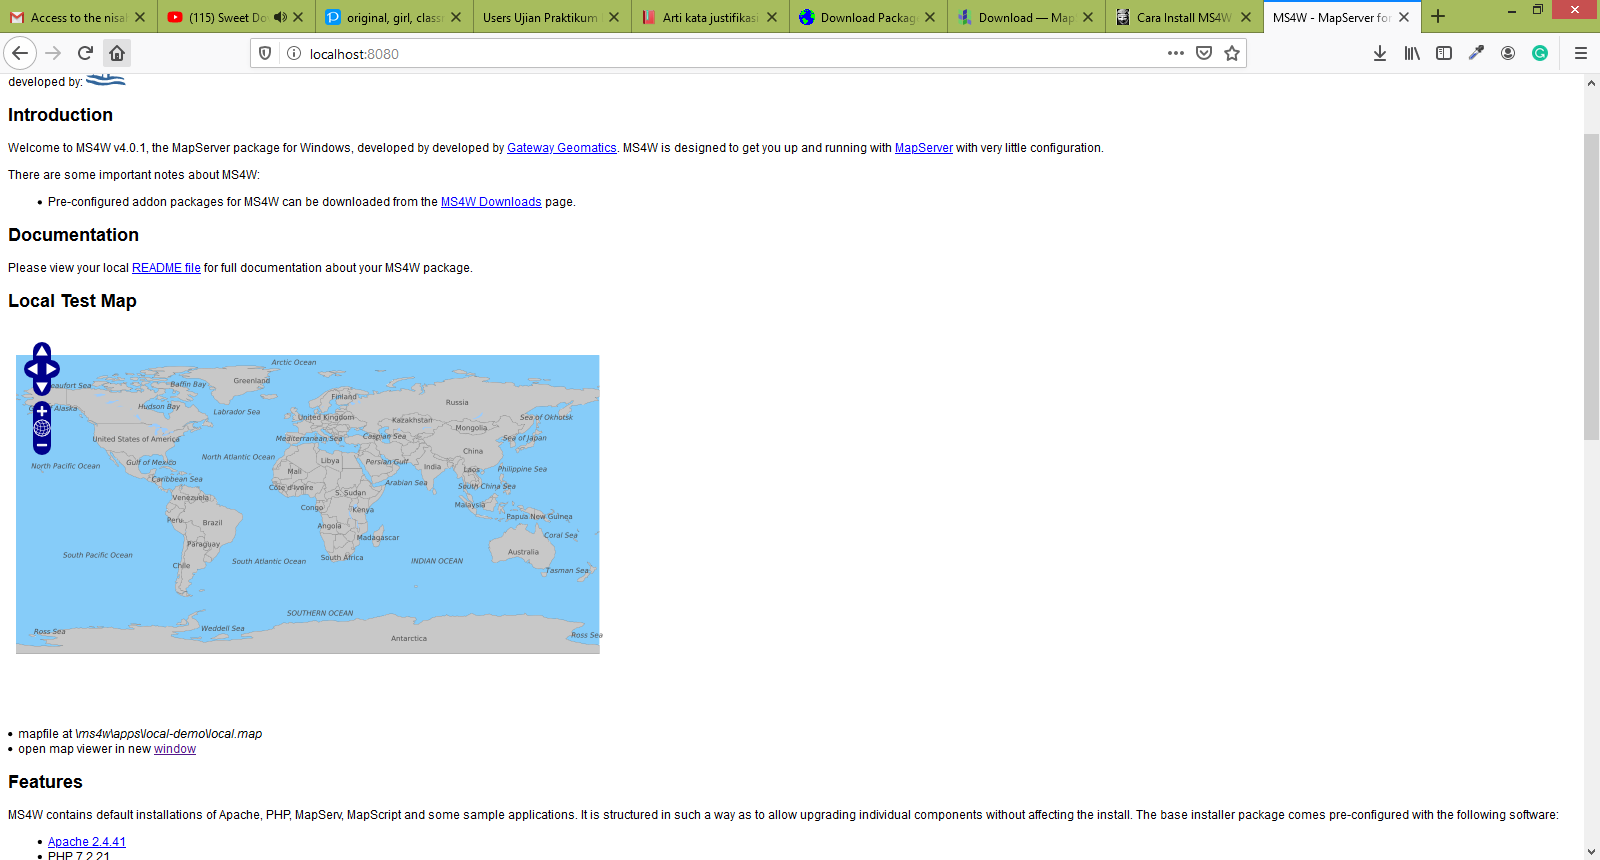
\includegraphics[width=8cm]{figures/1174035/tugas4/mapserver_5.png}
		\centering
		\caption{Hasil instalasi MS4w}
	\end{figure}
\end{enumerate}
\subsection{Mengkonfigurasi MapProxy}
MapProxy berfungsi untuk menampilkan file python yang dapat menampilkan peta. Berikut metode instalasi dan konfigurasinya :
\begin{enumerate}
    \item Buka command prompt
    \item Ketik "pip install mapproxy"
    \hfill\break
	\begin{figure}[H]
		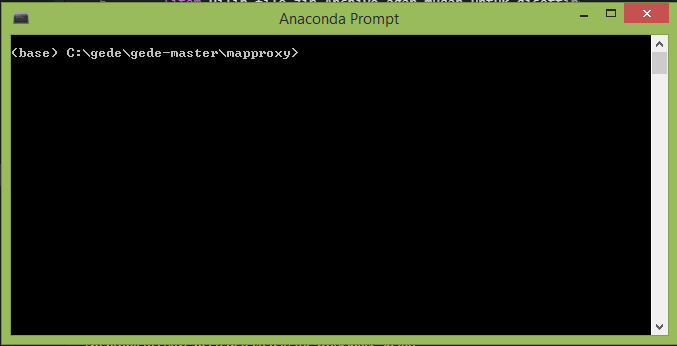
\includegraphics[width=8cm]{figures/1174035/tugas4/mapproxy_1.png}
		\centering
		\caption{Instalasi mapproxy di python}
	\end{figure}
    \item Setelah itu, pastikan mapproxy sudah dapat dicek versinya "mapproxy-util --version"
    \hfill\break
	\begin{figure}[H]
		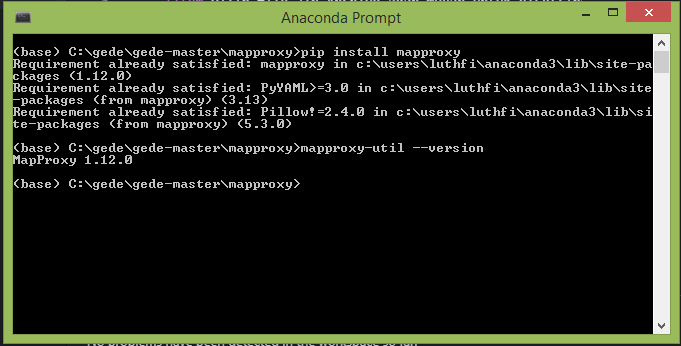
\includegraphics[width=8cm]{figures/1174035/tugas4/mapproxy_2.png}
		\centering
		\caption{Pengecekan versi mapproxy}
	\end{figure}

\end{enumerate}
\subsection{Mencoba Memakai File yaml}
File yaml akan dipakai untuk mengambil keseluruhan file map yang ada. Berikut metodenya : 
\begin{enumerate}
    \item Coba download file berikut \href{Awangga/Gede}{https://github.com/awangga/gede}
    \hfill\break
	\begin{figure}[H]
		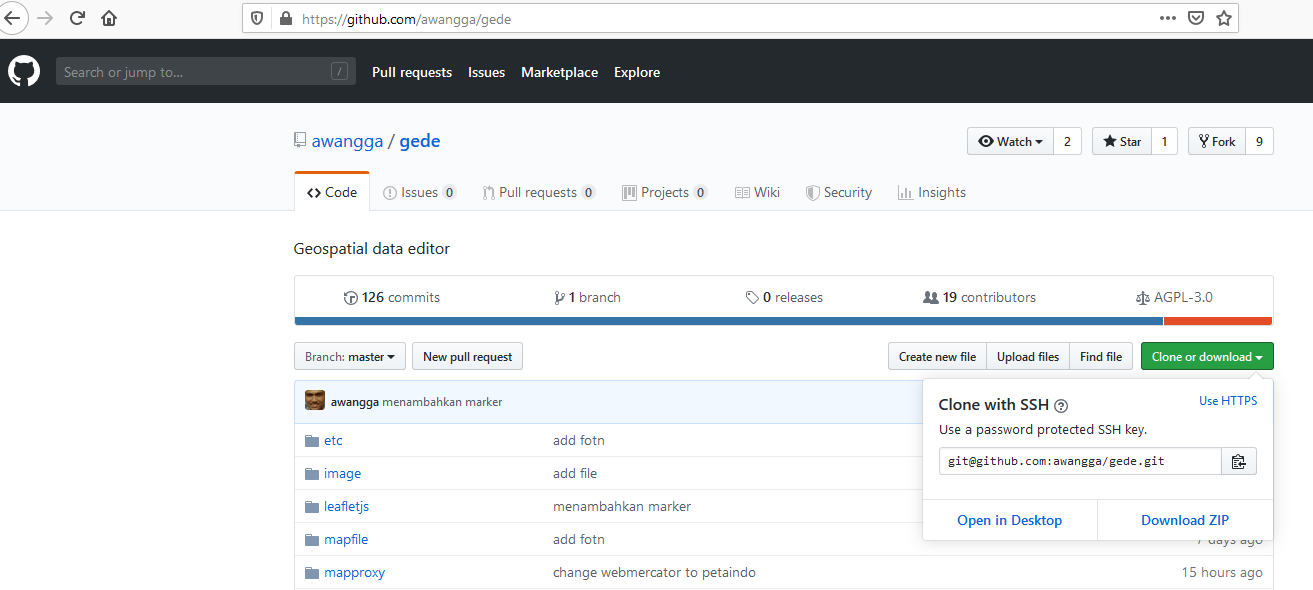
\includegraphics[width=8cm]{figures/1174035/tugas4/yaml_1.png}
		\centering
		\caption{Mendownload File Map}
	\end{figure}
    \item Extract file dimanapun
    \hfill\break
	\begin{figure}[H]
		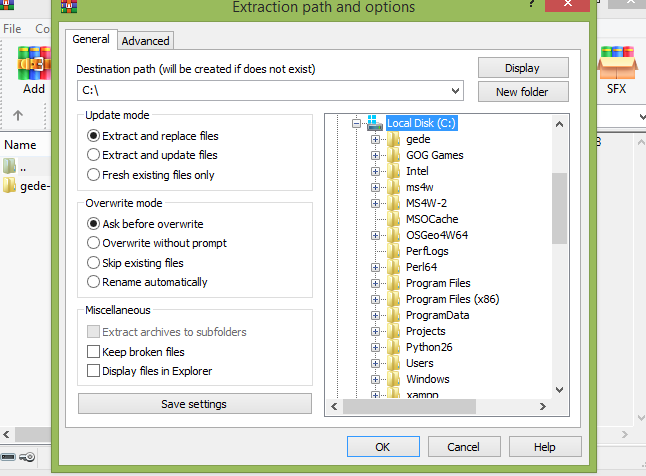
\includegraphics[width=8cm]{figures/1174035/tugas4/yaml_2.png}
		\centering
		\caption{Extract Hasil Download}
	\end{figure}
    \item Lalu pada command prompt, masuk ke folder lokasi extract/mapproxy
    \hfill\break
	\begin{figure}[H]
		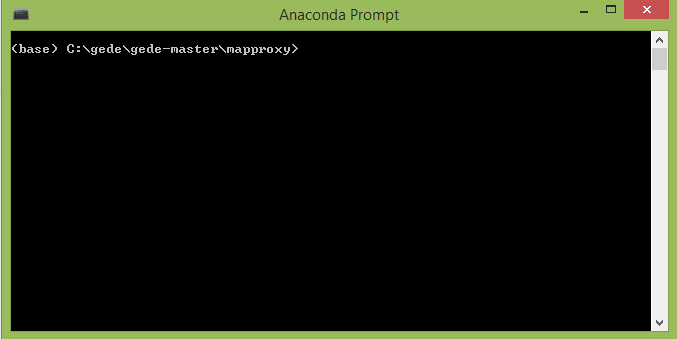
\includegraphics[width=8cm]{figures/1174035/tugas4/yaml_3.png}
		\centering
		\caption{Masuk lokasi file yang diextract pada cmd}
	\end{figure}
    \item Keluar dari command prompt (Jangan di exit), Edit file agm.yaml
    \hfill\break
	\begin{figure}[H]
		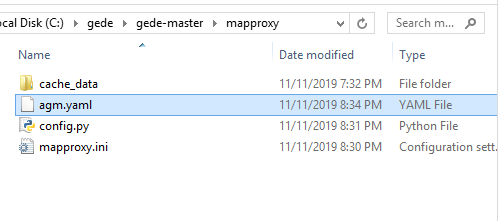
\includegraphics[width=8cm]{figures/1174035/tugas4/yaml_4.png}
		\centering
		\caption{File agm.yaml di folder mapproxy}
	\end{figure}
    \item Lalu edit file yaml pada bagian berikut : 
    \begin{itemize}
        \item Map : Ada pada folder mapfile di hasil yang di extract
        \item Binary : Ada pada lokasi file MS4W/Apache
        \item Working Dir : Ada pada di folder yang di extarct/tmp
    \end{itemize}
    \hfill\break
	\begin{figure}[H]
		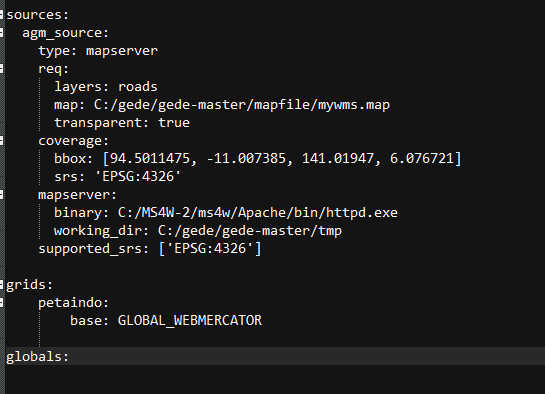
\includegraphics[width=8cm]{figures/1174035/tugas4/yaml_5.png}
		\centering
		\caption{Editing file yaml}
	\end{figure}
    \item Save dan kembali ke command prompt
    \item Tulis kode berikut "mapproxy-util serve-develop agm.yaml"
    \hfill\break
	\begin{figure}[H]
		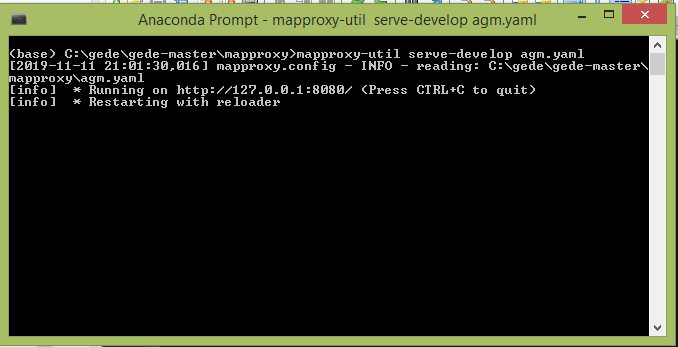
\includegraphics[width=8cm]{figures/1174035/tugas4/yaml_6.png}
		\centering
		\caption{Mencoba menjalankan mapproxy}
	\end{figure}
    \item Maka akan dapat dibuka langsung pada lokasi link \href{http://localhost:8080}{http://localhost:8080}
    \hfill\break
	\begin{figure}[H]
		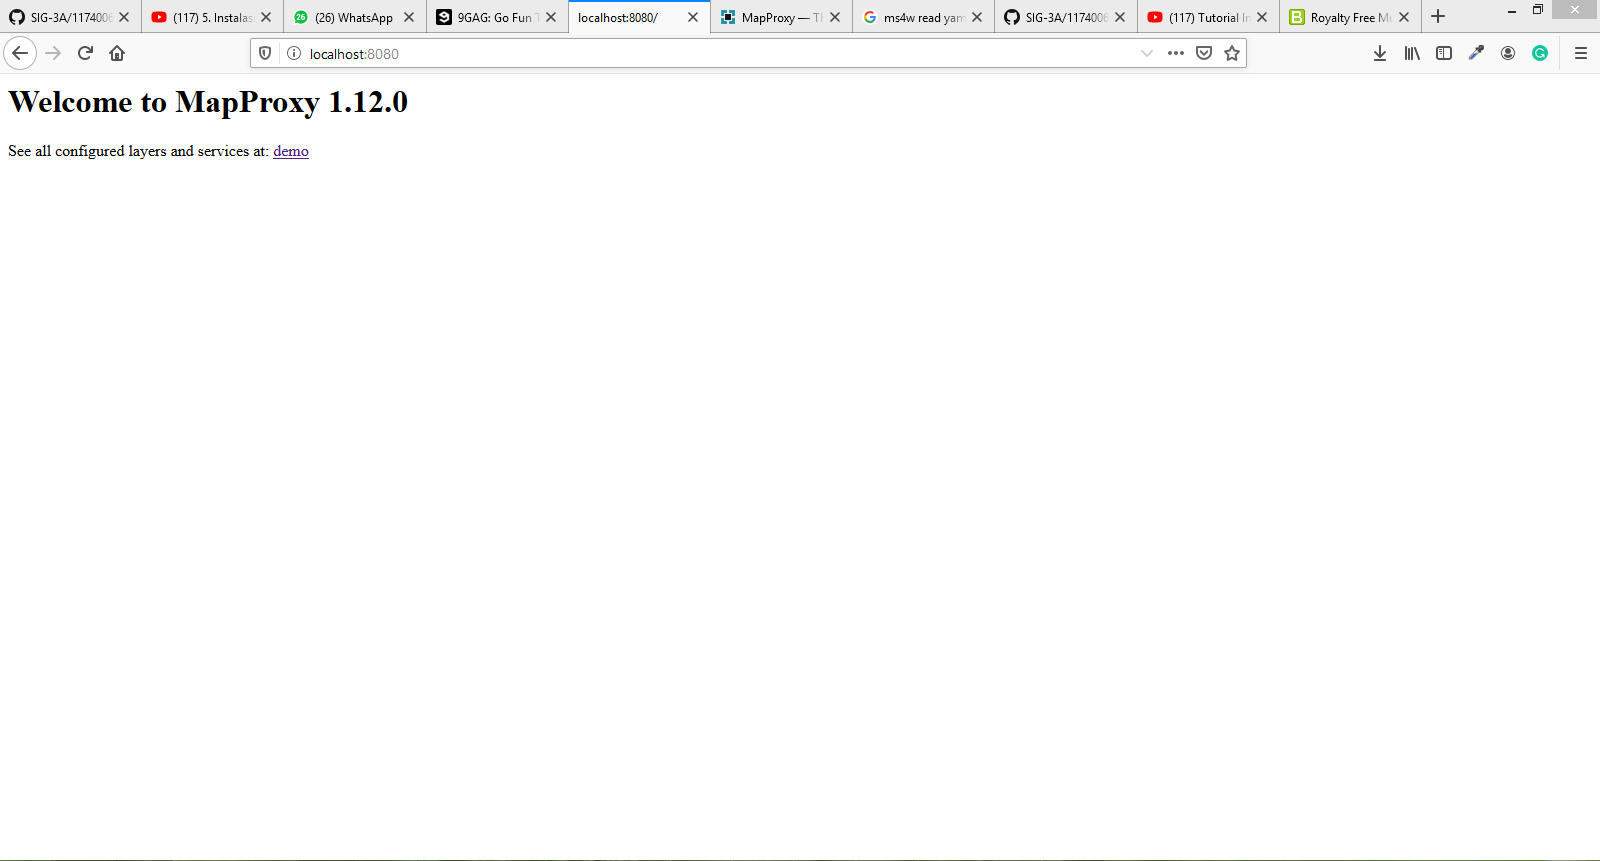
\includegraphics[width=8cm]{figures/1174035/tugas4/yaml_7.png}
		\centering
		\caption{Mencoba memanggil mapproxy pada browser}
	\end{figure}
\end{enumerate}
\subsection{Video Tutorial}
\href{https://youtu.be/7AzaqTXLK8A}{Link Youtube}
\subsection{Plagiarism Check}
\hfill\break
\begin{figure}[H]
    \includegraphics[width=8cm]{figures/1174035/tugas4/Plagiat.png}
    \centering
    \caption{Plagiat Check}
\end{figure}